%% LyX 2.3.3 created this file.  For more info, see http://www.lyx.org/.
%% Do not edit unless you really know what you are doing.
\documentclass[french]{extarticle}
\usepackage{fancyhdr}
\pagestyle{fancy}
\setcounter{secnumdepth}{4}
\usepackage{color}
\addtolength{\oddsidemargin}{-.8in}
\addtolength{\evensidemargin}{-.8in}
\addtolength{\textwidth}{1.6in}
\makeatletter
% \addto\extrasfrench{%
%    \providecommand{\og}{\leavevmode\flqq~}%
%    \providecommand{\fg}{\ifdim\lastskip>\z@\unskip\fi~\frqq}%
% }

\makeatother
\usepackage{graphicx}
\usepackage[unicode=true,pdfusetitle,
 bookmarks=true,bookmarksnumbered=false,bookmarksopen=false,
 breaklinks=false,pdfborder={0 0 0},pdfborderstyle={},backref=false,colorlinks=true]
 {hyperref}
\hypersetup{
 linkcolor=blue,urlcolor=blue}

\makeatletter
%%%%%%%%%%%%%%%%%%%%%%%%%%%%%% Textclass specific LaTeX commands.
\newcommand{\lyxrightaddress}[1]{
	\par {\raggedleft \begin{tabular}{l}\ignorespaces
	#1
	\end{tabular}
	\vspace{1.4em}
	\par}
}

%%%%%%%%%%%%%%%%%%%%%%%%%%%%%% User specified LaTeX commands.CONTINUE
% \usepackage{minted}

\usepackage[svgnames]{xcolor}
\usepackage{svg}
\usepackage{algorithmeUTF8}
\usepackage[utf8]{inputenc}

\usepackage{fancyhdr}
\lhead{TITRE DOCUMENT}
\chead{}
\rhead{}
\lfoot{AUTEURS - AUTEURS}
\cfoot{Page \thepage}
\rfoot{\today}
\usepackage{fancyvrb}
\renewcommand{\headrulewidth}{0.4pt}
\renewcommand{\footrulewidth}{0.4pt}
\addtolength{\headheight}{\baselineskip}

\makeatother

\begin{document}

\rhead{
\includegraphics[height=1cm]{./Rapport/Logo_INSARouen.png}}
\title{TITRE}
\author{AUTEURS - RU Siu - MELO DA SILVA Alexis - MESBAH Zacharia - SAIVRES
Jerôme - SI Ruixu}
\date{2019 - 2020}
\maketitle

\newpage{}

\tableofcontents{}\newpage{}

\section{TADs}
\documentclass[]{article}
\usepackage{babel}
\usepackage[utf8]{inputenc}
\usepackage{algorithmeUTF8} 
\begin{document}

	\begin{tad}
		\tadNom{Couleur}
		\tadDependances{Chaine de caractères}
		\begin{tadOperations}{Couleur}
			\tadOperation{Couleur}{\tadUnParam{Chaine de caractères}}{\tadUnParam{Couleur}}
			\tadOperation{CouleurOpposée}{\tadUnParam{Couleur}}{\tadUnParam{Couleur}}
			
		\end{tadOperations}
		\begin{tadAxiomes}
			\tadAxiome{CouleurOpposée( CouleurOpposée( Couleur ))) = Couleur}
		\end{tadAxiomes}
	\end{tad}
	
	\begin{tad}
		\tadNom{Pion}
		\tadDependances{Couleur}
		\begin{tadOperations}{Pion}
			\tadOperation{Pion}{\tadUnParam{Couleur}}{\tadUnParam{Pion}}
			\tadOperation{ObtenirCouleur}{\tadUnParam{Pion}}{\tadUnParam{Couleur}}
			\tadOperation{InverserCouleur}{\tadUnParam{Pion}}{\tadUnParam{Pion}}
		\end{tadOperations}
		\begin{tadAxiomes}
			\tadAxiome{InverserCouleur(InverserCouleur(Pion(Couleur))) = Pion}
		\end{tadAxiomes}
	\end{tad}
	
	\begin{tad}
		\tadNom{Position}
		\tadDependances{Colonne,Ligne}
		\begin{tadOperations}{Position}
			\tadOperation{Position}{\tadUnParam{Colonne x Ligne}}{\tadUnParam{Position}}
			\tadOperation{FixerColonne}{\tadUnParam{Colonne}}{\tadUnParam{Position}}
			\tadOperation{FixerLigne}{\tadUnParam{Ligne}}{\tadUnParam{Position}}
			\tadOperation{ObtenirColonne}{\tadUnParam{Position}}{\tadUnParam{Colonne}}
			\tadOperation{ObtenirLigne}{\tadUnParam{Position}}{\tadUnParam{Ligne}}
		\end{tadOperations}
		\begin{tadAxiomes}
		\end{tadAxiomes}
	\end{tad}
	
	\begin{tad}
		\tadNom{Coup}
		\tadDependances{Position,Pion,Plateau}
		\begin{tadOperations}{Coup}
			\tadOperation{Coup}{\tadUnParam{Position x Pion}}{\tadUnParam{Coup}}
			\tadOperation{ObtenirPosition}{\tadUnParam{Coup}}{\tadUnParam{Position}}
			\tadOperation{ObtenirPion}{\tadUnParam{Coup}}{\tadUnParam{Pion}}
			\tadOperation{EstValideCoup}{\tadUnParam{Plateau}}{\tadUnParam{Booleen}}
		\end{tadOperations}
		\begin{tadAxiomes}
		\end{tadAxiomes}
	\end{tad}
	
	\begin{tad}
		\tadNom{Plateau}
		\tadDependances{Position,Coup,Plateau,Pion}
		\begin{tadOperations}{Plateau}
			\tadOperation{Plateau}{\tadUnParam{Naturel x Naturel}}{\tadUnParam{Plateau}}
			\tadOperation{JouerCoup}{\tadUnParam{Plateau x Coup}}{\tadUnParam{Plateau}}
			\tadOperation{ObtenirPion}{\tadUnParam{Plateau x Position}}{\tadUnParam{Pion}}
			\tadOperation{CaseVide}{\tadUnParam{Plateau x Position}}{\tadUnParam{Booleen}}
			\tadOperation{Remplacer}{\tadUnParam{Plateau x Position}}{\tadUnParam{Plateau}}
		\end{tadOperations}
		\begin{tadAxiomes}
			\tadAxiome{ObtenirPion(JouerCoup(Plateau,Coup(Position,Pion)), Position) = Pion}
			\tadAxiome{Remplacer(Remplacer(Plateau,Position),Position) = Plateau}
		\end{tadAxiomes}
	\end{tad}
	
	\begin{tad}
		\tadNom{Coups}
		\begin{tadOperations}{Coups}
			\tadOperation{Coups}{}{\tadUnParam{Ensemble<Coup>}}
			\tadOperation{AjouterCoup}{\tadUnParam{Coups x Coup}}{\tadUnParam{Coups}}
			\tadOperation{RetirerCoup}{\tadUnParam{Coups x Coup}}{\tadUnParam{Coups}}
			\tadOperation{NombreCoups}{\tadUnParam{Coups}}{\tadUnParam{Naturel}}
		\end{tadOperations}
		
	\end{tad}
	
\end{document}

\section{Analyse Descendante}
\begin{figure}[h]
  \centering
  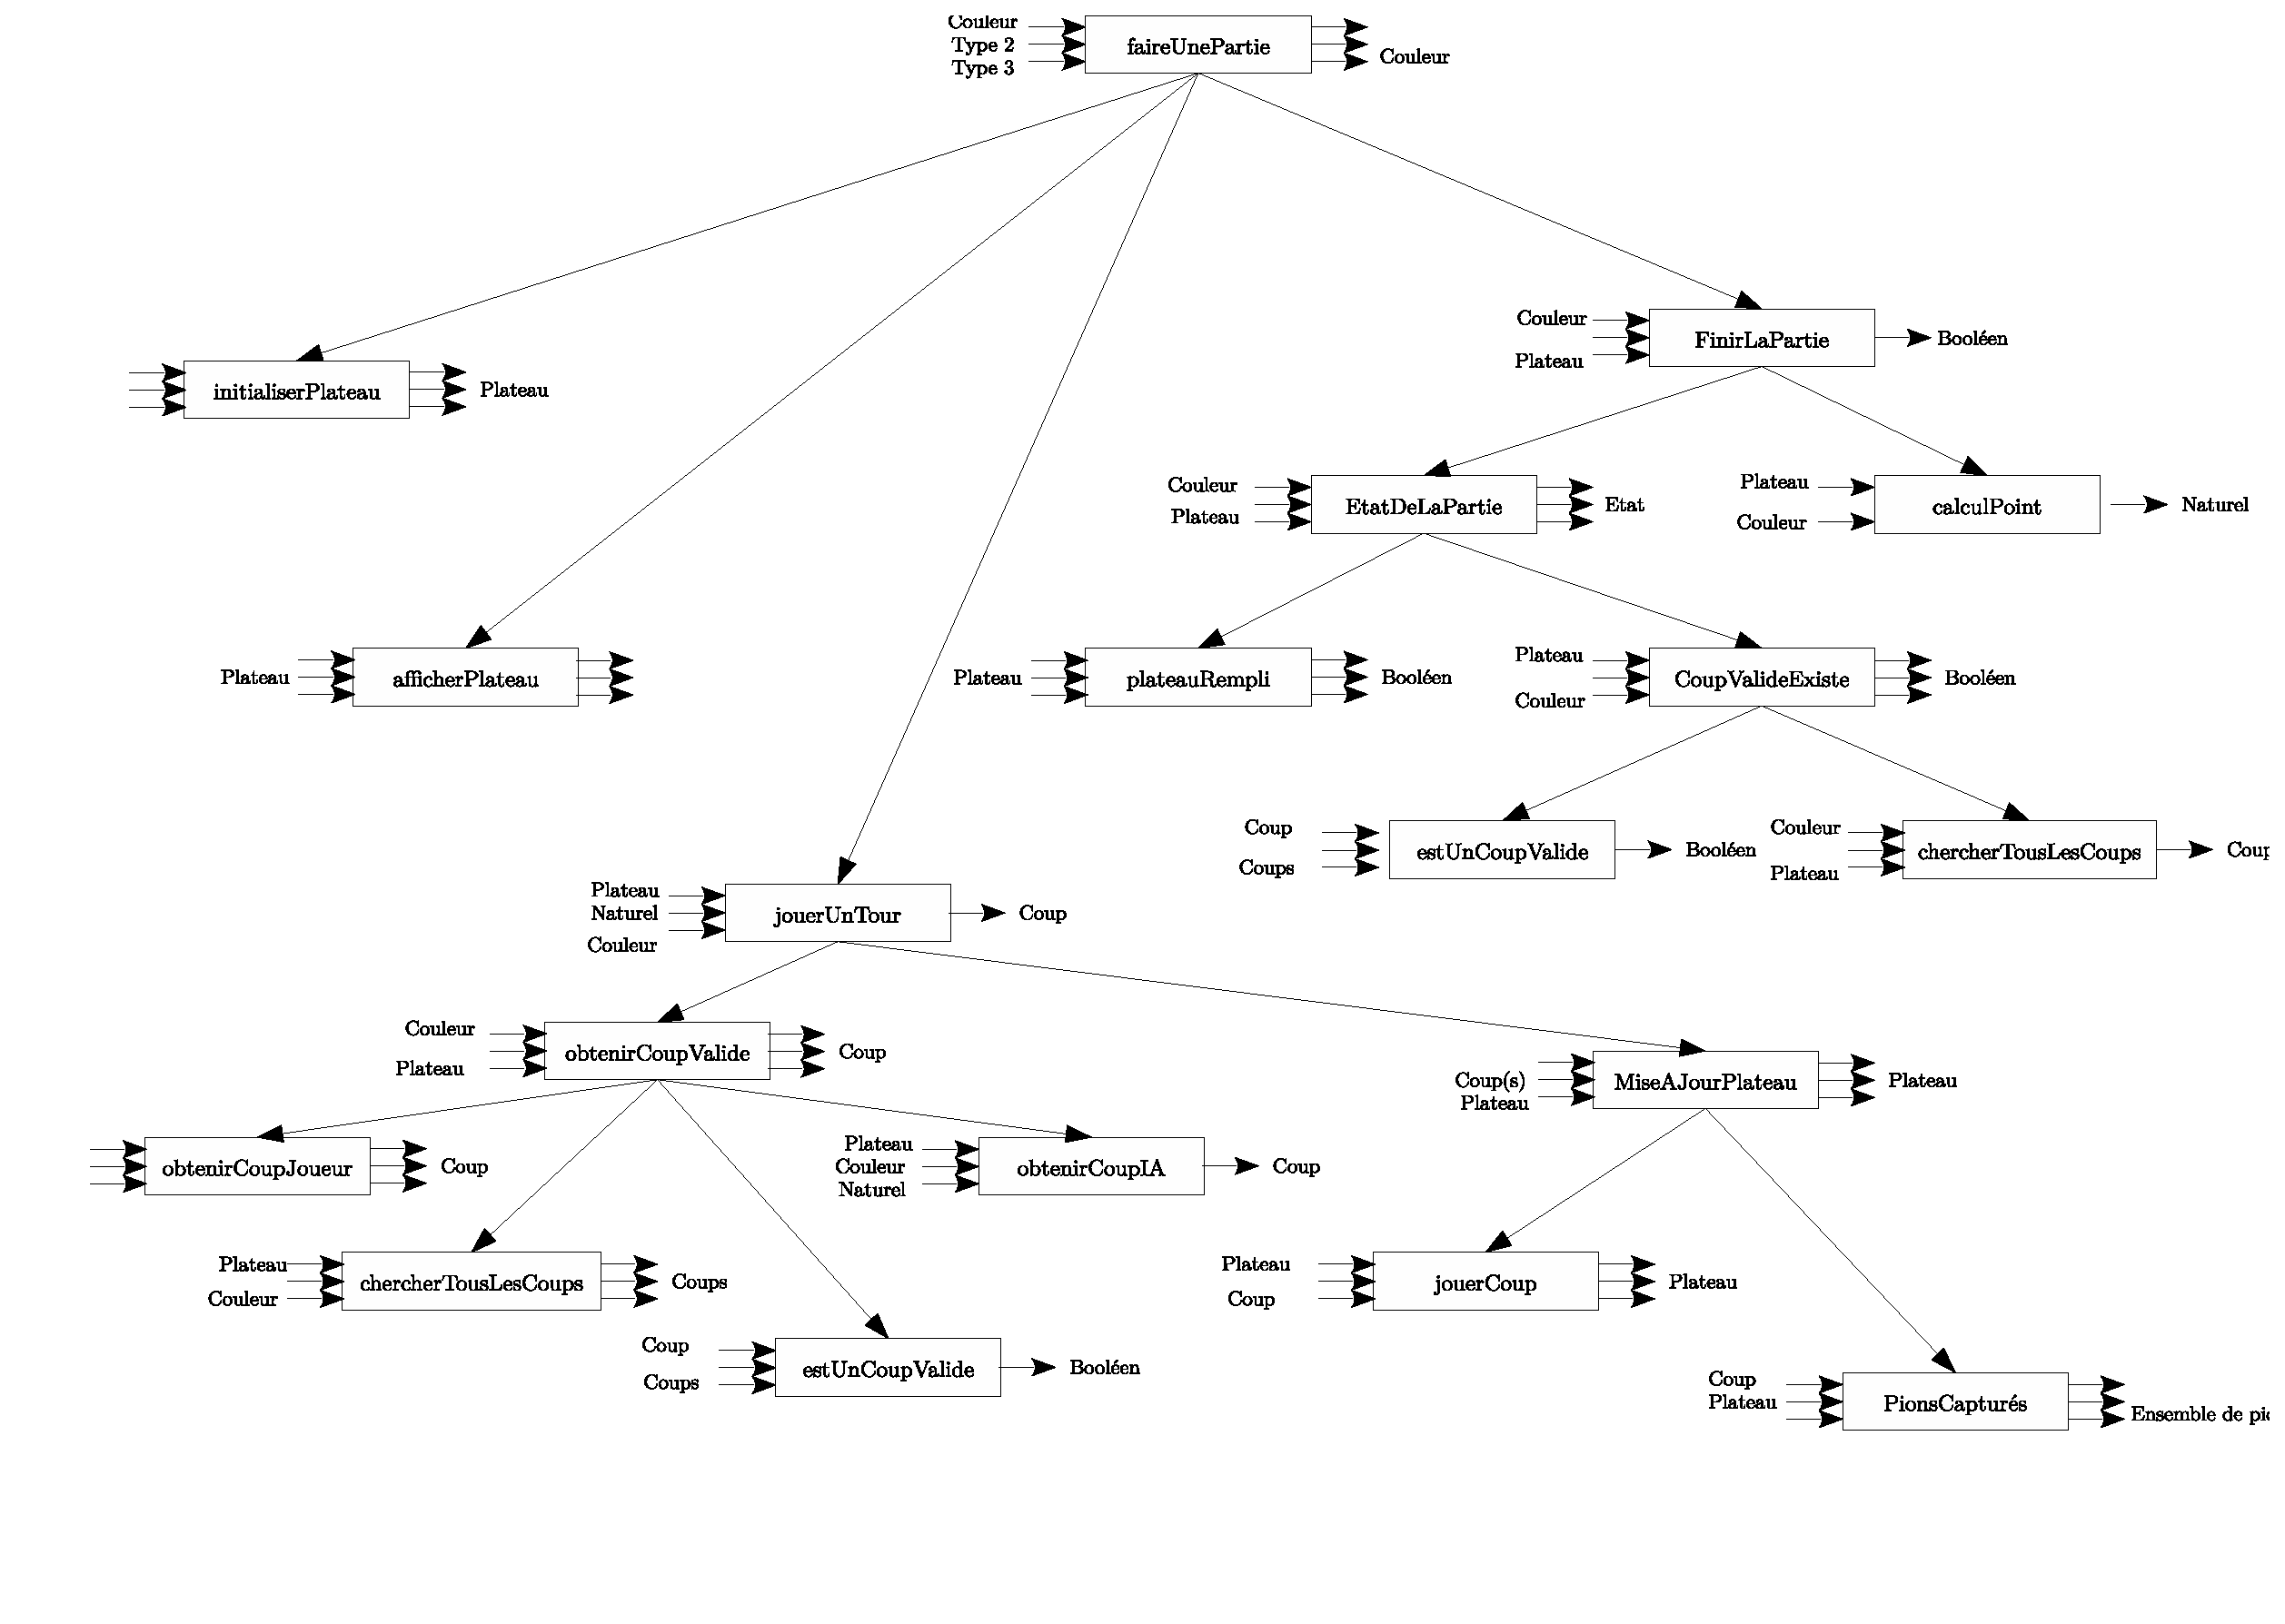
\includegraphics[scale = 0.2]{./Rapport/Analyse_descendante.eps}
  \caption{Analyse descendante}
  \includegraphics[scale = 0.2]{./Rapport/Analyse_descendante_jouer_un_tour.eps}
  \caption{Analyse descendante jouer un tour}
\end{figure}
\newpage
\section{Conception détaillée}
\subsection{Signatures}
	\signatureprocedure {jouerUnePartie}{Couleur}
	\signaturefonction {InitialiserPlateau}{None}{Plateau}
	\signatureprocedure {AfficherPlateau}{Plateau}
	\signaturefunction {JouerUnTour}{Plateau, Naturel, Couleur}{Coup}
	\signaturefunction {obtenirCoupValide}{Couleur, Plateau}{Coup}
	\signaturefunction {obtenirCoupIA}{Plateau, Couleur, Naturel}{Coup}
	\signaturefunction {obtenirCoupJoueur}{}{Coup}
	\signaturefunction {estUnCoupValide}{Coup, Coups}{Booléen}
	\signaturefunction {chercherTousLesCoups}{Plateau, Couleur}{Coups}
	\signaturefunction {MiseAJourPlateau}{Coup, Plateau}{Plateau}
	\signaturefunction {jouerCoup}{Plateau, Coup}{Plateau}
	\signaturefunction {PionsCapturés}{coup, Plateau}{Ensemble de pion}
	\signaturefunction {finirLaPartie}{Couleur, Plateau}{Naturel}
	\signaturefunction {EtatDeLaPartie}{Couleur, Plateau}{Etat}
	\signaturefunction {CalculPoint}{Couleur, Plateau}{Naturel}
	\signaturefunction {plateauRempli}{Plateau}{Booléen}
	\signaturefunction {CoupValideExiste}{Plateau, Couleur}{Booléen}
\section{Types}
\begin{algorithme}

	\begin{enregistrement}{Couleur}
		\champEnregistrement{nom}{Chaine de caractères}
		\champEnregistrement{hexa}{Chaine de caractères}
		\champEnregistrement{couleurOpposee}{Couleur}
		\champEnregistrement{symbole}{Caractère}
	\end{enregistrement}
\\	
	\begin{enregistrement}{Pion}
		\champEnregistrement{couleur}{Couleur}
	\end{enregistrement}
\\
	\begin{enregistrement}{Position}
		\champEnregistrement{ligne}{Ligne}
		\champEnregistrement{colonne}{Colonne}
	\end{enregistrement}
\\

	\begin{enregistrement}{Coup}
		\champEnregistrement{pion}{Pion}
		\champEnregistrement{position}{Position}
	\end{enregistrement}
\\\\	
	\textbf{Type} Plateau \textbf{=} tableau[1...longueur][1...longueur] de Pions
\\\\
	\textbf{Type} Coups \textbf{=} Ensemble<Coup>
\\\\
	\textbf{Type} Ligne \textbf{=} Entier[1...longueur]
\\\\
	\textbf{Type} Colonne \textbf{=} Entier[1...longueur] 
	
\end{algorithme}



\end{document}
